\documentclass[mirror, portugues]{revdetua}
%
% Valid options are:
%   portugues --------- main language is Portuguese
%   final ------------- final version (default)
%   times ------------- use times (postscript) fonts for text
%   mirror ------------ prints a mirror image of the paper (with dvips)
%   visiblelabels ----- \SL, \SN, \SP, \EL, \EN, etc. defined
%   invisiblelabels --- \SL, \SN, \SP, \EL, \EN, etc. not defined (default)
%
% Note: the final version should use the times fonts
% Note: the really final version should also use the mirror option

\usepackage[portuguese]{babel}
\usepackage[utf8]{inputenc}
\usepackage{amsmath} 
\usepackage{comment}
\usepackage{algorithm}
\usepackage{algpseudocode}
\floatname{algorithm}{Algoritmo}
\usepackage{graphicx}
\usepackage[justification=centering]{caption}
\usepackage{float}
%-------------------------------------
% compiling:
% Recipe: xelatex
% Recipe: pdflatex -> bibtex -> pdflatex -> pdflatex
% Recipe: xelatex
%
% notas:
% rever se algorimtos e imagens estão onde devem
%-------------------------------------
\begin{document}

\Header{02}{3}{Dezembro}{2024}{1}

\title{Maximum Weight Cut Problem}
% MUDAR TITULO ALLEZ ALLEZ ALGO COM RANDOMIZADO
\author{Hugo Veríssimo - 124348 - hugoverissimo@ua.pt}
\maketitle

\begin{abstract}
... abstrato em ingles
% por fazer abstrato
\end{abstract}

\begin{resumo}
Este relatório apresenta a implementação e comparação de dois métodos para resolver o problema \textit{Maximum Weight Cut}: uma pesquisa exaustiva e uma heurística gulosa. O problema \textit{Maximum Weight Cut} con ESTE É O ANTIGO FAZER NOVO
\end{resumo}

\section{Introdução}

O problema \textit{Maximum Weight Cut} é um problema de otimização, que tem como objetivo encontrar o corte mais pesado num grafo não direcionado $G(V,E)$, onde $|V| = n$ vértices e $|E| = m$ arestas. Este corte envolve dividir os vértices do grafo em dois subconjuntos disjuntos $S$ e $T$, sendo que o corte é a soma dos pesos das arestas que ligam os vértices de $S$ aos vértices de $T$: $|E(S, T)|$ \cite{AG14}.

No passado relatório foram analisados algoritmos determinísticos para resolver o problema \textit{Maximum Weight Cut}, nomeadamente a pesquisa exaustiva e a heurística gulosa. Neste relatório, serão analisados novos algoritmos com um certo grau de estocasticidade, com o objetivo de encontrar um algortimo que otimize o equilíbrio entre a complexidade computacional e a qualidade da solução obtida.

% POR ACABAR INTRO
para alem disso os resultados são comparados aos obtidos anteriormente

serao entao implexmentados 3 algoritmos, nomeadamente: ... e ...

DIZER ALGURES Q O NUMERO DE OPERACOES SERA A METRICA USADA PARA CONFIRMAR A COMPLEXIDADE DOS ALGORTIMO

\section{Metodologia da Análise}

Com o intuito de analisar o problema em destaque, implementar os algoritmos referidos e comparar os resultados obtidos, foi utilizada a linguagem de programação \textit{Python}, devido à vasta variedade de bibliotecas que contém, facilitando a implementação eficiente e simplificada dos algoritmos necessários.

% ACABAR ISTO, CORRIGIR COM OS PRINCIPAIS Q USAR REALMENTE
Sem desmerecer o uso de ficheiros auxiliares, a análise desenvolvida pode ser dividida em 2 ficheiros principais, sendo estes:
\begin{verbatim}
    $ python3 benchmarks.py
\end{verbatim}
% .......

Para a realização da análise dos algoritmos criados, foram utilizados grafos gerados aleatoriamente, com a semente $124348$, com diferentes números de vértices e densidade de arestas, e os grafos da coleção \textit{Gset}, disponibilizada por Yinyu Ye \cite{GS24}.

\section{Algoritmo de Corte Aleatório}

O primeiro algoritmo a ser implementado é um algoritmo de corte aleatório, que consiste em gerar várias soluções aleatórias e comparar as mesmas, escolhendo a melhor solução \cite{AG14}.

Este será um algortimo computacionalmente leve, pela sua simplicidade, mas não garante a obtenção da solução ótima, devido à sua natureza aleatória, sendo que a probabilidade de encontrar a mesma, assumindo que é única, é dada por

$$1 - \left( 1 - \frac{1}{2^{n-1}} \right)^{solutions}$$

\noindent onde $n$ é o número de vértices e $solutions$ é o número de soluções a gerar. Pode-se facilmente verificar que, para grafos de grandes dimensões, esta probabilidade decresce exponencialmente, tornando o algoritmo cada vez menos preciso.

Pelo facto do algoritmo gerar muitas soluções aleatórias, é importante garantir que não existem soluções repetidas a ser testadas, para evitar o cálculo do peso do corte, uma operação computacionalmente cara. Para isso é criado um \textit{set} onde serão guardadas as soluções já testadas, e cada vez que uma solução for gerada, a mesma só será testada depois de ser verificado que não é uma repetição. 

Atendendo à paragem do algoritmo, este tem dois critério de paragem, parando assim que um deles é verificado. O primeiro, e mais provável em grafos de grandes dimensões, é quando o número de soluções geradas atinge o limite, definido pelo utilizador. O segundo critério, é verificado quando todas as soluções possíveis foram testadas, ou seja, quando o \textit{set} que acompanha as soluções testadas contém $2^n$ elementos.

Este algoritmo pode ser então traduzido para o seguinte pseudocódigo:

\begin{algorithm}[H]
\raggedright
\textbf{Entrada:}

- lista de arestas e respetivos pesos (\textit{edges})

- número de vértices (\textit{n\_nodes})

- número de soluções a gerar (\textit{solutions})\\
\textbf{Saída:} subconjuntos \textit{S} e \textit{T}, peso do corte (\textit{weight}) \\
\hrule 
\caption{Corte Aleatório}
\begin{algorithmic}[1]
    \State \texttt{best\_solution} $\gets$ \texttt{None}
    \State \texttt{weight} $\gets$ 0
    \State \texttt{seen\_solutions} $\gets$ empty set
    \For{$i \gets 1$ \textbf{to} \texttt{solutions}}
        \State \texttt{partition} $\gets$ random partition of the nodes
        \If {\texttt{length}(\texttt{seen\_solutions}) $=$ $2^{\texttt{n\_nodes}}$}
            \State \textbf{break}
        \EndIf
        \State \texttt{partition\_hash} $\gets$ hash the partition
        \If {\texttt{partition\_hash} $\in$ \texttt{seen\_solutions}}
            \State \textbf{continue}
        \EndIf
        \State Add \texttt{partition\_hash} to \texttt{seen\_solutions}
        \State \texttt{new\_cut\_weight} $\gets$ compute the cut weight
        \If {\texttt{new\_cut\_weight} $>$ \texttt{weight}}
            \State \texttt{weight} $\gets$ \texttt{new\_cut\_weight}
            \State \texttt{best\_solution} $\gets$ copy of \texttt{partition}
        \EndIf
    \EndFor
    \State \texttt{S} $\gets$ set of nodes assigned to $0$ in \texttt{best\_solution}
    \State \texttt{T} $\gets$ set of nodes assigned to $1$ in \texttt{best\_solution}
    \Return \texttt{S}, \texttt{T}, \texttt{weight}
\end{algorithmic}
\end{algorithm}
    
Pode-se observar que a parte computacionalmente mais custosa deste algoritmo é o ciclo, que é responsável por gerar cortes aleatórios e calcular o peso dos mesmos. A complexidade deste ciclo é dado por $O(n + m)$, por percorrer todos os vértices atribuindo-as a um dos subconjuntos, e por calcular o peso do corte, percorrendo todas as arestas. Assim, a complexidade final do algoritmo é dada por $O((n + m) \times \texttt{solutions})$, visto que o ciclo corre no máximo \texttt{solutions} vezes. Esta complexidade pode ser simplifcada para $O(m)$, visto que $m \gg n$ para grafos densos e um $n$ grande, e que \texttt{solutions} é uma constante.

\begin{figure}[H]
    \centering
    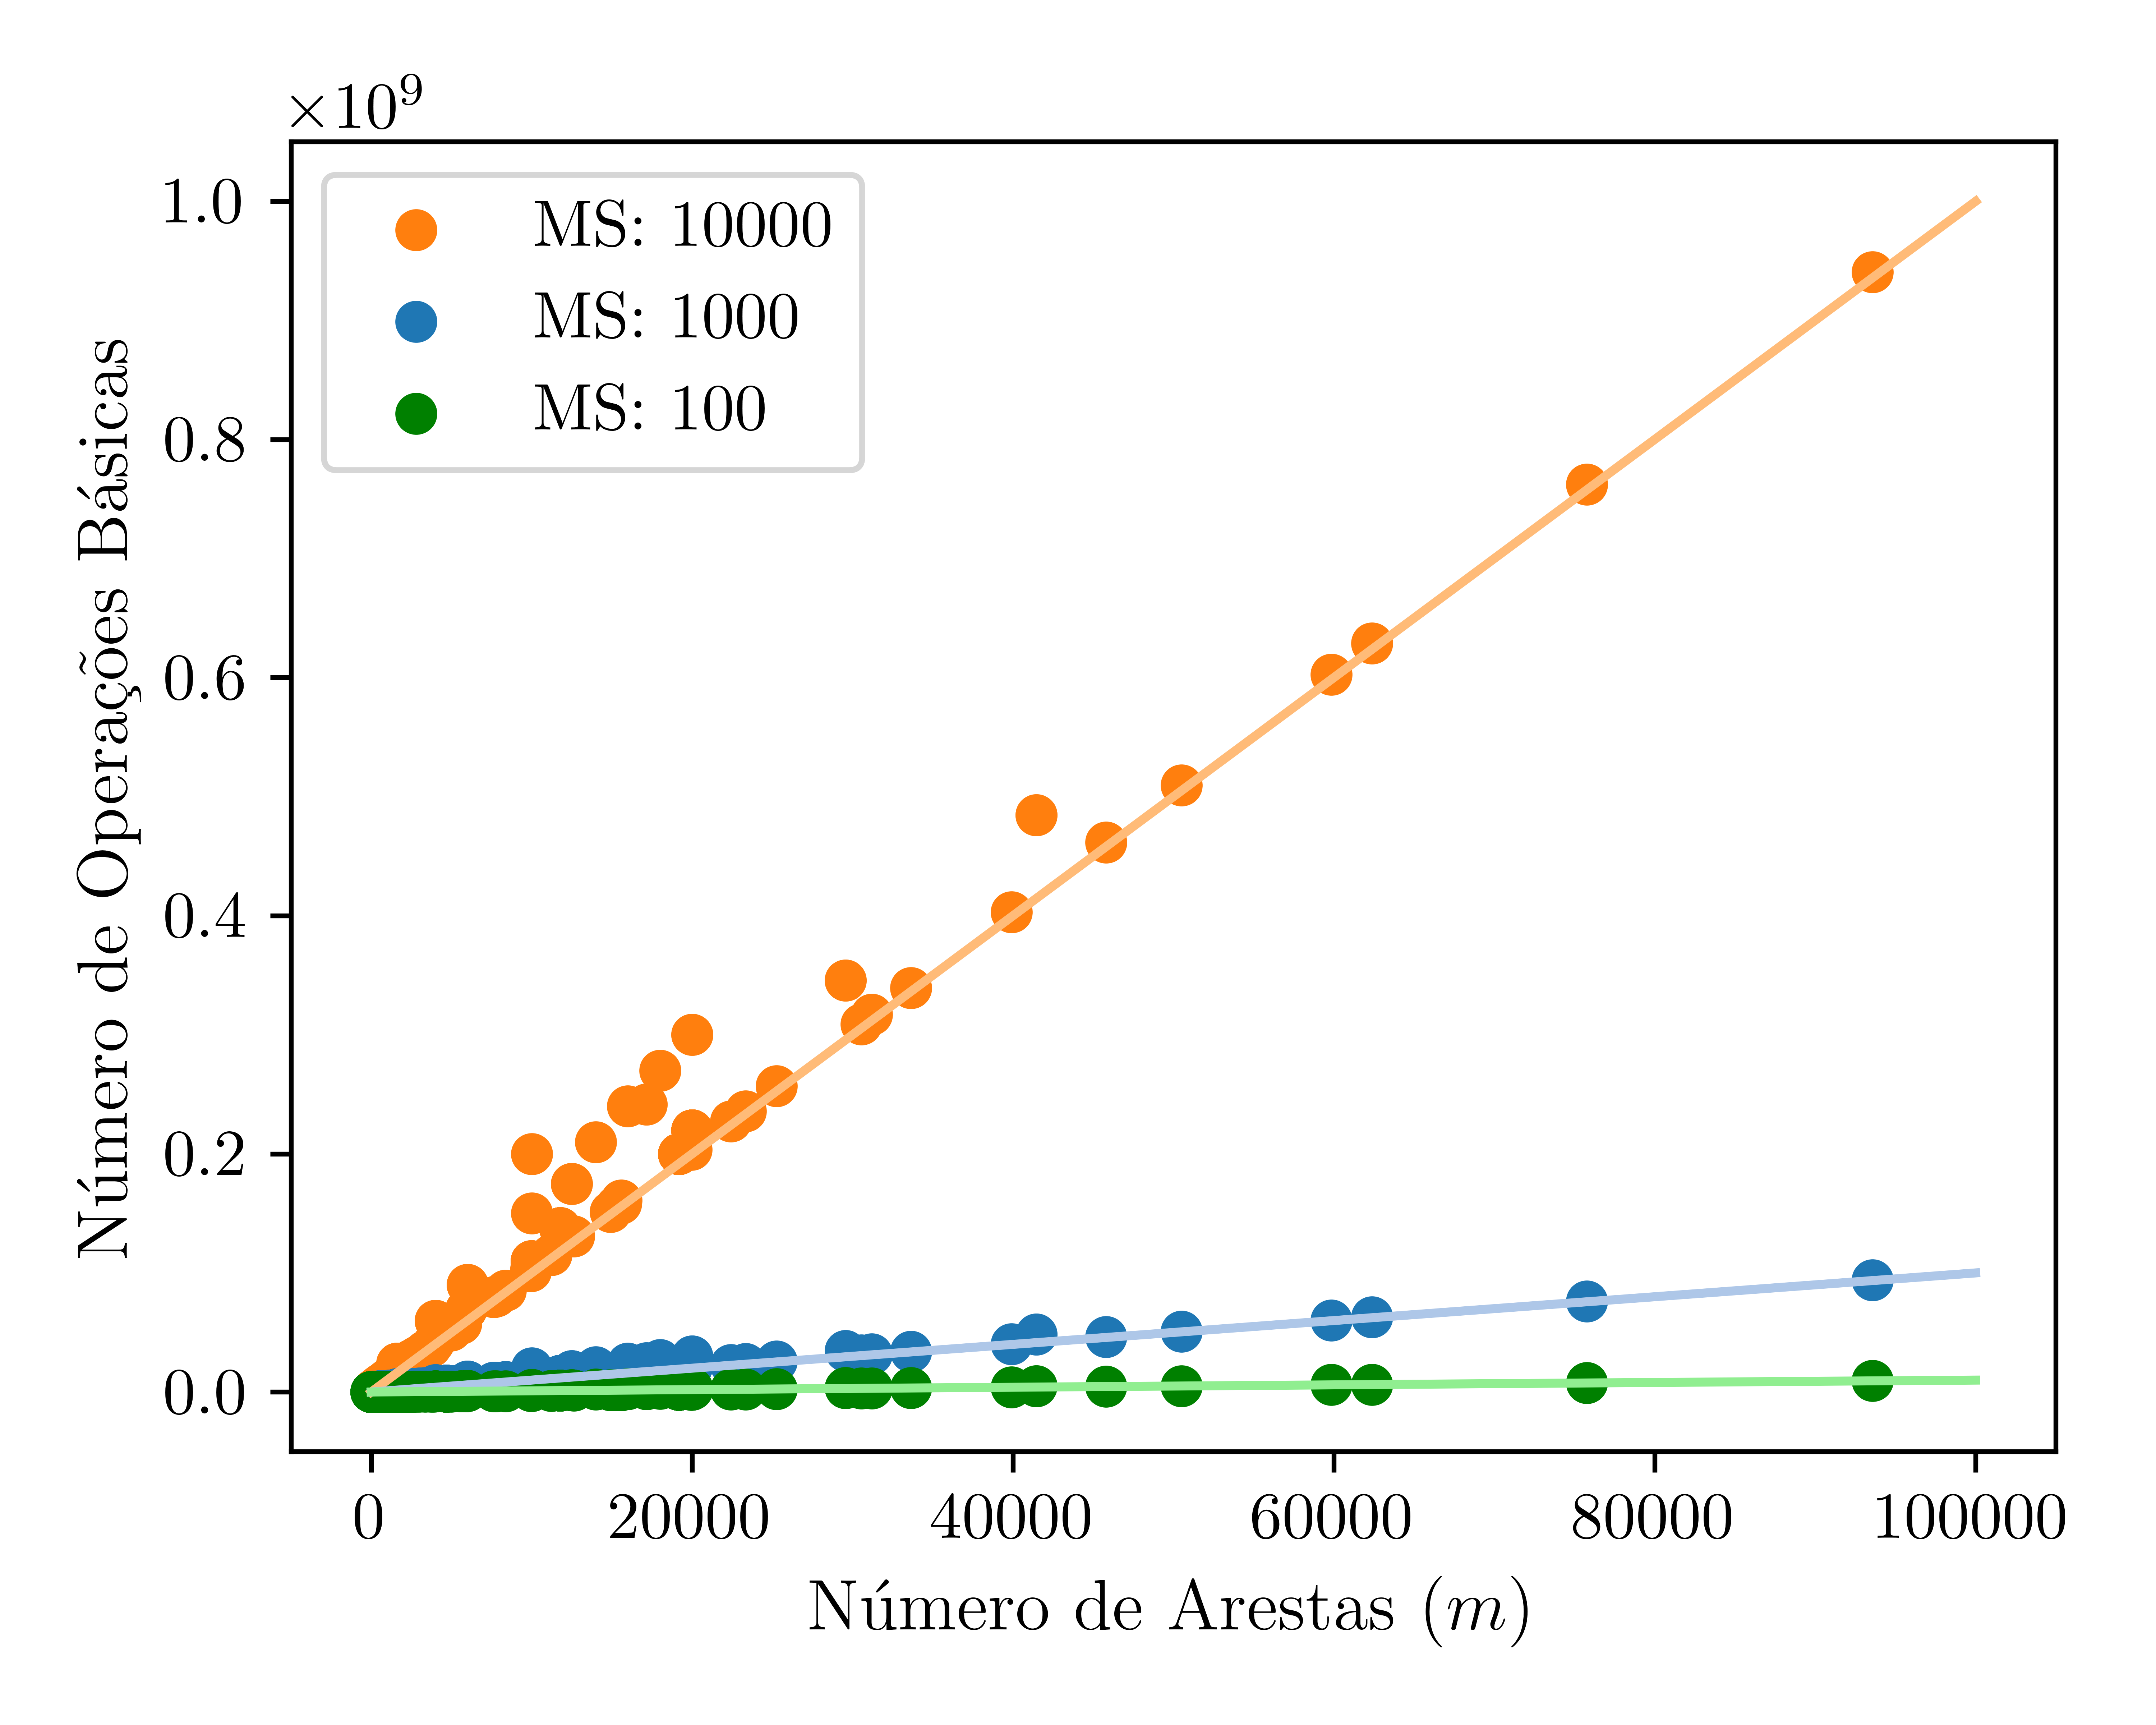
\includegraphics[width=0.45\textwidth]{../assets/ops_Random Sol.png}
    \caption{camptionsdasid8}
    \label{fig:random_ops}
\end{figure}

A complexidade referida é confirmada pela análise experimental apresentada na figura \ref{fig:random_ops}, onde se pode observar que o número de de operações básicas realizadas é linear em relação ao número de arestas do grafo, para diferentes números de soluções geradas.

% dizer q é m * solutions no grafico e q os pontos acima do reta tem a ver com qnd o m não é mt maior q n, mas que em grafos densos pronto

% dizer que o algortimo e mais rapido e isso qnd ms é 100 e coisas assim



\section{Algoritmo de Simulated Annealing}

O segundo algoritmo a ser implementado é o algoritmo de \textit{Simulated Annealing} (SA), uma heurística de pesquisa aleatória, que consiste em encontrar soluções aproximadas para problemas de otimização combinatória \cite{SAT15}. Este método consite em gerar uma solução inicial aleatória, e a partir desta solução, gerar soluções vizinhas, que são soluções obtidas a partir da solução atual, e comparar as soluções, aceitando as soluções melhores e algumas piores, com uma probabilidade que decresce ao longo das iterações, até que a temperatura (parâmetro do algoritmo), que vai arrefecendo ao longo das iterações a uma determinada taxa de arrefecimento (paraâmetro do algoritmo), seja menor que um determinado valor, por exemplo $10^{-3}$, sendo este o critério de paragem do algoritmo \cite{SA87}.

Assim, é possível verificar que este algortimo tem como componente aleatória a seleção de uma solução inicial e a aceitação de soluções piores, e como parte determinística a diminuição da probabilidade de aceitação de soluções piores ao longo das iterações e a garantia de aceitação de soluções melhores.

Na figura \ref{fig:sa_aceitacao}, pode-se observar o comportamento decrescente da probabilidade de aceitação de soluções piores ao longo das iterações do algoritmo SA. Os pontos cinzentos representam números aleatórios gerados dentro do intervalo $[0,1]$ a cada iteração. A proposta de uma nova solução é aceite se esta for melhor que a solução atual ou se o valor aleatório (ponto cinzento) estiver abaixo da "curva" definida pelos pontos azuis. Esta curva reflete a probabilidade de aceitação, que diminui à medida que a temperatura decresce, limitando cada vez mais a aceitação de soluções subótimas.

\begin{figure}[H]
    \centering
    \includegraphics[width=0.45\textwidth]{../assets/SA_DecrAceit.png}
    \caption{Probabilidade de aceitação de uma solução subótima, em função do número de iterações, quando o SA é aplicado com a semente $124348$, ao grafo G59.}
    \label{fig:sa_aceitacao}
\end{figure}

É também importante referir que o algoritmo não garante a não repetição de soluções previamente testadas, e não foi implementado um mecanismo para tal, visto que a probabilidade de testar a mesma solução é baixa para grafos de grandes dimensões, e o processo de comparação de soluções já testadas poderia prejudicar a eficiência do algoritmo.

% probabilidade de testar duas vezes a mesma solucao ?
% em 1 passo, n/n * 1/n
% 4 passos, n/n * 1/n * n-1/n * 1/n
% ....

O algoritmo de \textit{Simulated Annealing} pode ser examinado em detalhe no seguinte pseudocódigo:

\begin{algorithm}[H]
\raggedright
\textbf{Entrada:}

- lista de arestas e respetivos pesos (\textit{edges})

- temperatura (\textit{Temp})

- taxa de arrefecimento (\textit{cooling\_rate})\\
\textbf{Saída:} subconjuntos \textit{S} e \textit{T}, peso do corte (\textit{best\_cut}) \\
\hrule 
\caption{\textit{Simulated Annealing}}
\begin{algorithmic}[1]
    \State \texttt{partition} $\gets$ random partition of the nodes
    \State \texttt{best\_partition} $\gets$ \texttt{partition}
    \State \texttt{current\_cut} $\gets$ compute the cut weight
    \State \texttt{best\_cut} $\gets$ \texttt{current\_cut}
    \While{\texttt{Temp} \ensuremath{>} \ensuremath{10^{-3}}}
        \State \texttt{node} $\gets$ randomly select a node
        \State Flip the partition of \texttt{node} in \texttt{partition}
        \State \texttt{new\_cut} $\gets$ compute the new cut weight
        \State \texttt{cost\_diff} $\gets$ \texttt{new\_cut} $-$ \texttt{current\_cut}
        \If{\texttt{cost\_diff} \ensuremath{>} 0 \textbf{or} random number $\in$ [0, 1] \ensuremath{<} $e^{\ensuremath{\texttt{cost\_diff} / \texttt{Temp}}}}$
            \Comment Accept the move
            \State \texttt{current\_cut} $\gets$ \texttt{new\_cut}
            \If{\texttt{new\_cut} \ensuremath{>} \texttt{best\_cut}}
                \State \texttt{best\_cut} $\gets$ \texttt{new\_cut}
                \State \texttt{best\_partition} $\gets$ \texttt{partition}
            \EndIf
        \Else
            \Comment Reject the move
            \State Revert the partition of \texttt{node} in \texttt{partition}
        \EndIf
        \State \texttt{Temp} $\gets$ \texttt{Temp} \ensuremath{\times} \texttt{cooling\_rate}
    \EndWhile
    \State \texttt{S} $\gets$ set of nodes assigned to $0$ in \texttt{best\_partition}
    \State \texttt{T} $\gets$ set of nodes assigned to $1$ in \texttt{best\_partition} \\
    \Return \texttt{S}, \texttt{T}, \texttt{best\_cut}
\end{algorithmic}
\end{algorithm}

Tal como foi referido na descrição do algoritmo, pode-se verificar que este é sensível à solução inicial, pelo que será interessante executar o algoritmo várias vezes, cobrindo uma maior área do espaço de soluções.

Para além disso, através do pseudocódigo, é possível analisar a complexidade do algoritmo em questão. As operações computacionalmente mais custosas encontram-se dentro do ciclo, que só termina após a temperatura ser inferior a $10^{-3}$. Assim, torna-se importante calcular o total de iterações ($k$) que o ciclo irá realizar, o que pode ser feito através da seguinte equação:

\begin{align*}
    &\texttt{Temp}_0 \cdot (\texttt{cooling\_rate})^k \le 10^{-3} \\
    \Leftrightarrow\ &  k \geq  \frac{\log\left(\frac{10^{-3}}{\texttt{Temp}_0}\right)}{\log(\texttt{cooling\_rate})} \\
    \Leftrightarrow\ & k = \left\lceil \frac{\log\left(\frac{10^{-3}}{\texttt{Temp}_0}\right)}{\log(\texttt{cooling\_rate})} \right\rceil
\end{align*}

\noindent Quanto à complexidade dentro do ciclo, a mesma é dada por $O(m)$, visto que a operação mais custosa é o cálculo do peso do corte, que percorre todas as arestas do grafo. Assim, a complexidade final do algoritmo é dada por $O(m \times k)$, e pelo facto de $k$ depender apenas da temperatura inicial e da taxa de arrefecimento, a complexidade final pode ser aproximada por $O(m)$.


\begin{figure}[H]
    \centering
    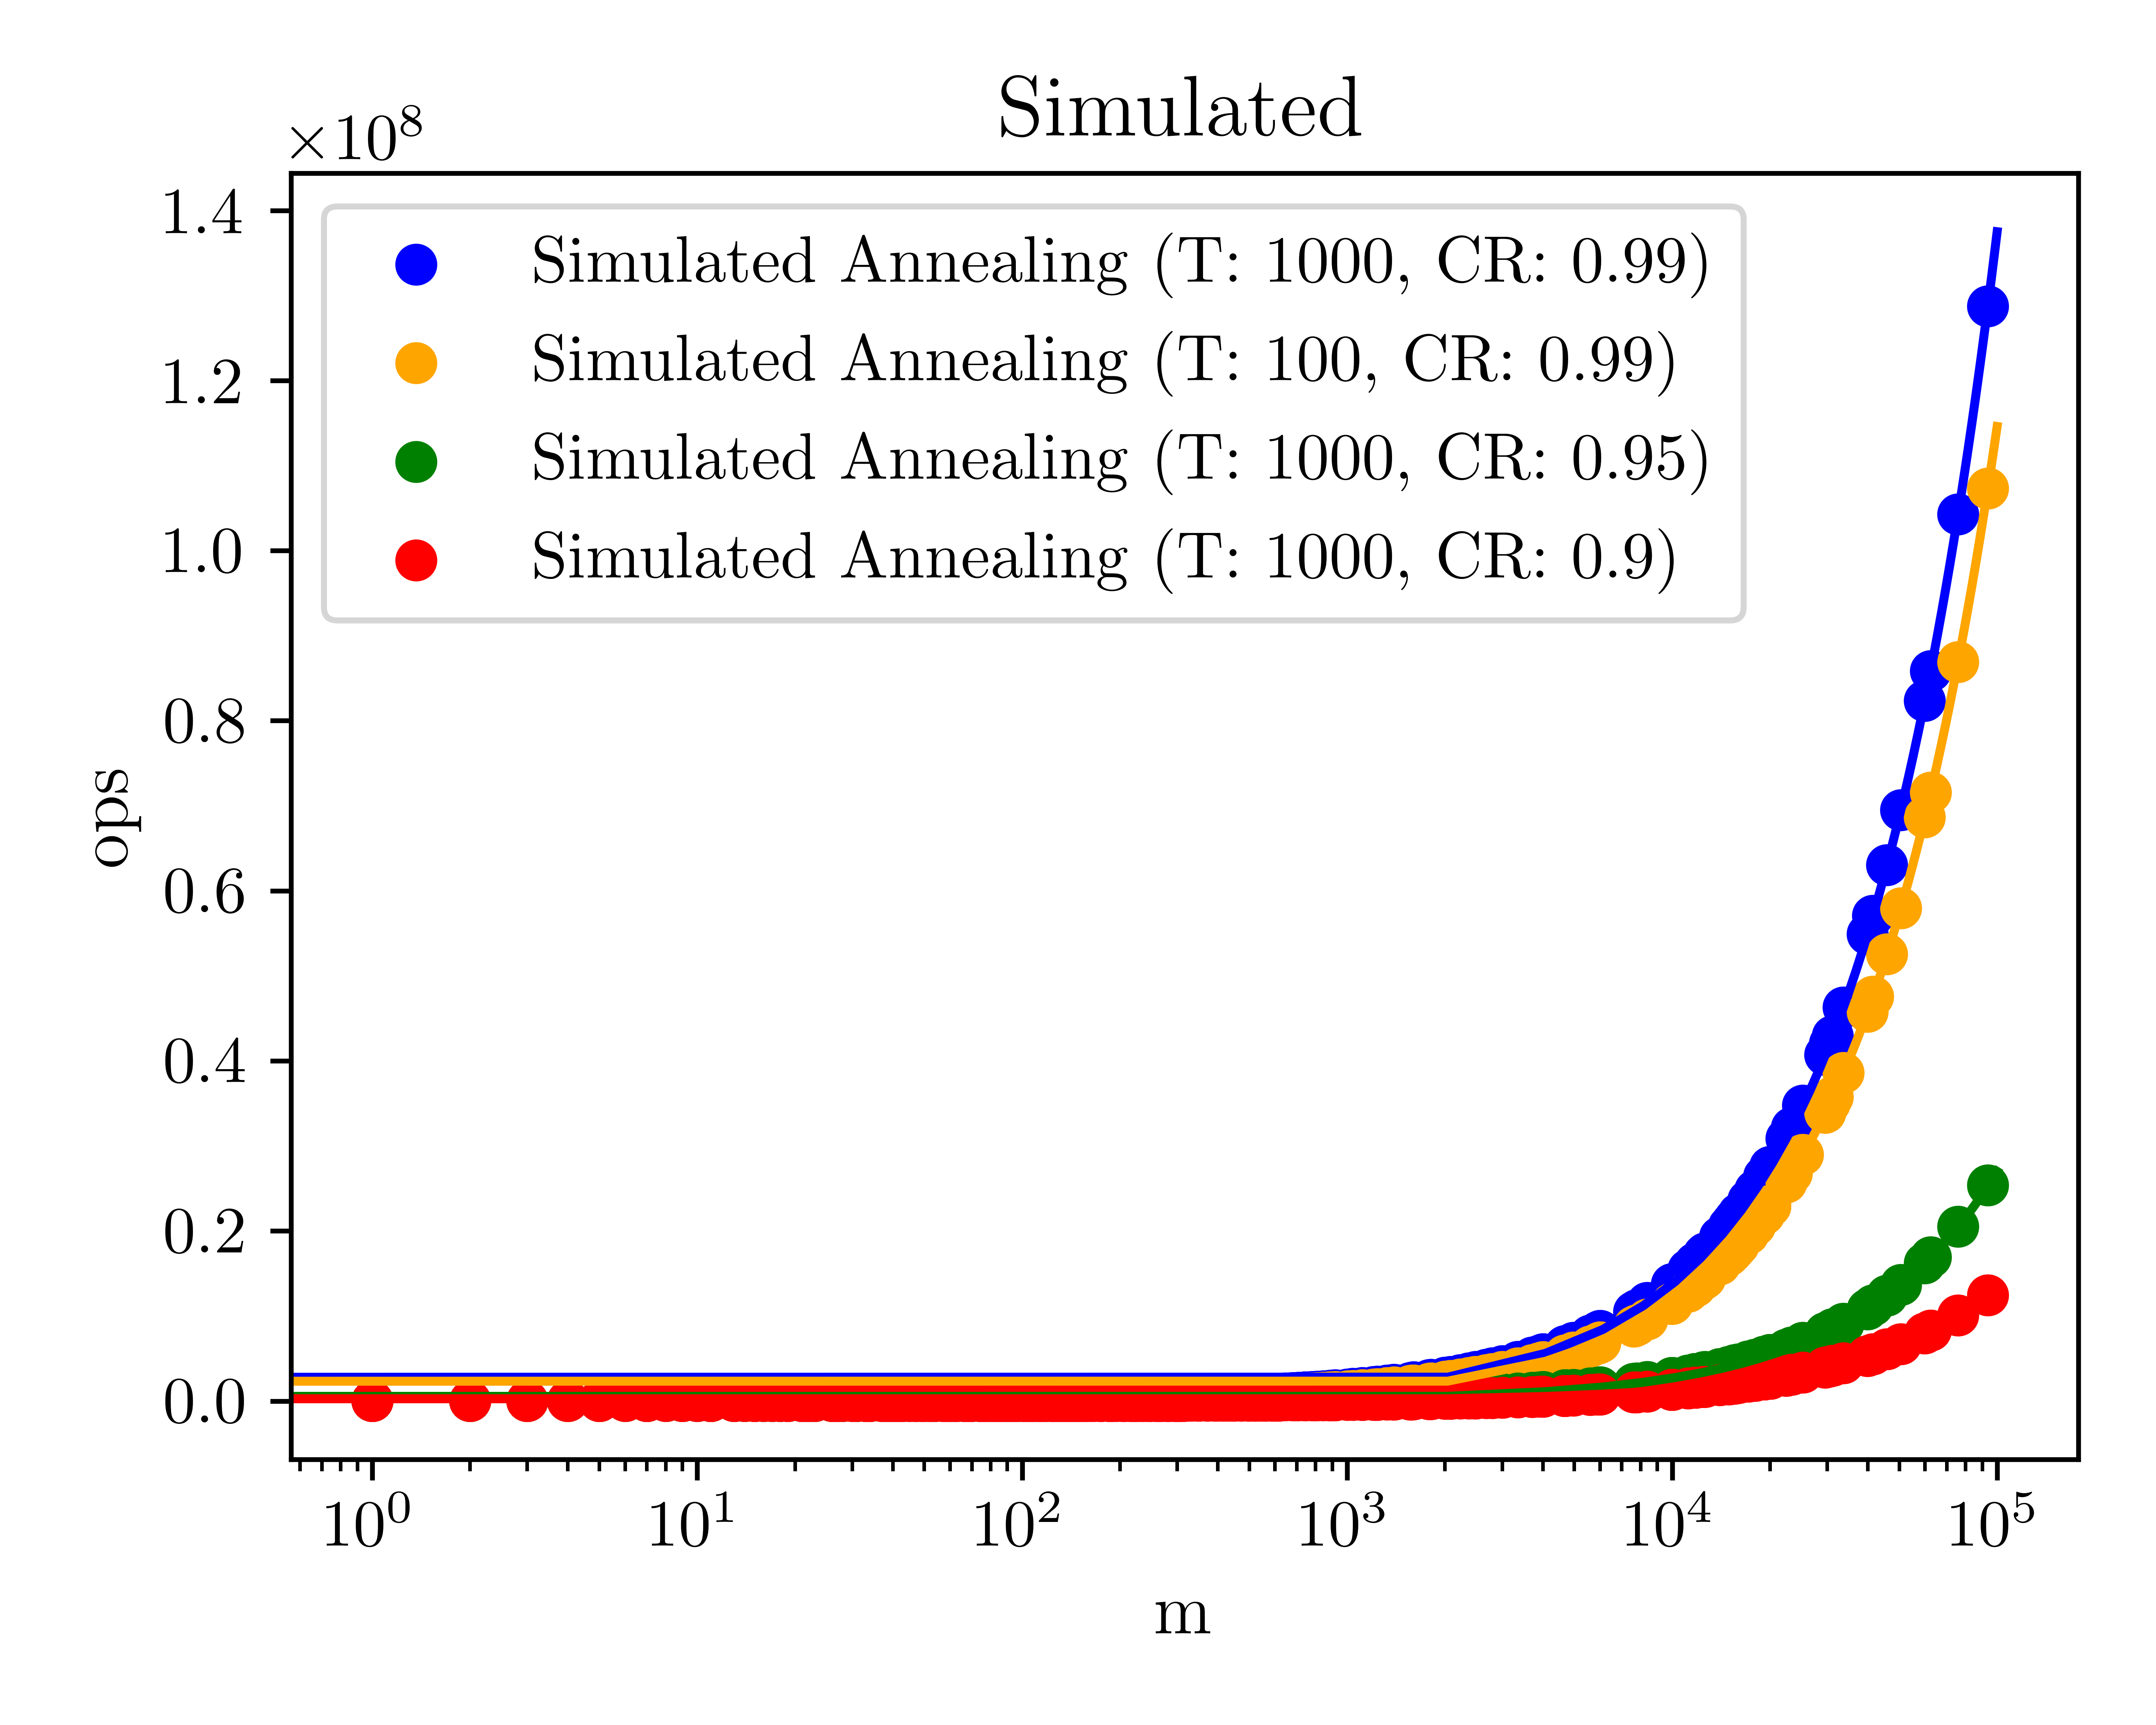
\includegraphics[width=0.45\textwidth]{../assets/ops_Simulated .png}
    \caption{camptionsdasid8}
    \label{fig:sa_ops}
\end{figure}


Através da figura \ref{fig:sa_ops} que representa o número de operações básicas realizadas em função do número de arestas do grafo, para diferentes temperaturas iniciais e taxas de arrefecimento, pode-se verificar que a complexidade do algoritmo é linear em relação ao número de arestas do grafo, para diferentes temperaturas iniciais e taxas de arrefecimento.

% falar a dizer q t maior implica... e cr maior implica ...


\section{Algoritmo Guloso Aleatório}

Por fim, o terceiro algoritmo a ser implementado é um algoritmo guloso aleatório, que segue uma heurística baseada numa abordagem gulosa, não garantido encontrar a solução ótima. Este algoritmo itera sobre todos os vértices do grafo e, para cada vértice, troca a sua partição, verificando se a nova configuração melhora a solução atual. Caso o peso do corte com o vértice na partição oposta seja maior que o atual, a solução é atualizada. O processo continua até que uma iteração completa seja realizada sem encontrar melhorias, momento em que o algoritmo termina.

Devido ao critério de paragem do algoritmo, este pode correr indefinidamente, devido à natureza aleatória da solução inicial, que pode estar a um grande número de iterações da solução estável que o algoritmo procura. Por isso, é adicionado um fator de ajuste do máximo de iterações (\textit{itLim}) ao algoritmo, tornando o número máximo de iterações do mesmo $m \times itLim$.

É também importante referir que, pelo factor na única componente aleatória deste algoritmo ser a criação de uma solução inicial, e como todas as iterações realizam alterações em direção à melhor solução, o algoritmo nunca irá testar a mesma solução mais que uma vez, pelo que manter um registo sobre as soluções já testadas não é necessário.

Este algoritmo pode ser representado em pseudocódigo da seguinte forma:

\begin{algorithm}[H]
\raggedright
\textbf{Entrada:}

- lista de arestas e respetivos pesos (\textit{edges})

- número de vértices (\textit{n\_nodes})

- fator de ajuste do máximo de iterações (\textit{itLim})\\
\textbf{Saída:} subconjuntos \textit{S} e \textit{T}, peso do corte (\textit{weight}) \\
\hrule 
\caption{Guloso Aleatório}
\begin{algorithmic}[1]
    \State \texttt{partition} $\gets$ random partition of the nodes
    \State \texttt{cut\_weight} $\gets$ compute the cut weight
    \State \texttt{improved} $\gets$ \texttt{True}
    \State \texttt{it\_limit} $\gets$ \texttt{len(edges)} \ensuremath{\times} \texttt{itLim}

    \While{\texttt{improved} \textbf{and} \texttt{it\_limit} \ensuremath{>} 0}
        \State \texttt{it\_limit} $\gets$ \texttt{it\_limit} $ - 1$
        \State \texttt{improved} $\gets$ \texttt{False}
        \For{\texttt{node} \textbf{in} \texttt{range}(\texttt{n\_nodes})}
            \State Flip the partition of \texttt{node} in \texttt{partition}
            \State \texttt{new\_cut\_weight} $\gets$ compute the cut weight
            \If{\texttt{new\_cut\_weight} \ensuremath{>} \texttt{cut\_weight}}
                \State \texttt{cut\_weight} $\gets$ \texttt{new\_cut\_weight}
                \State \texttt{improved} $\gets$ \texttt{True}
                \State \textbf{break}  \Comment{Stop iteration for this node}
            \EndIf
            \State Revert the partition of \texttt{node} in \texttt{partition}
        \EndFor
    \EndWhile

    \State \texttt{S} $\gets$ Set of nodes assigned to $0$ in \texttt{partition}
    \State \texttt{T} $\gets$ Set of nodes assigned to $1$ in \texttt{partition}
    \Return \texttt{S}, \texttt{T}, \texttt{cut\_weight}
\end{algorithmic}
\end{algorithm}

% AQUIIIIIIIII

como o algoritmo é guloso, a solucao final depende da solucao inicial, gerada aleatoriamente, e por isso o algoritmo deve ser corrido varias vezes, para garantir uma maior probabilidade a melhor solucao é encontrada
    
quanto a compelxidade, gerar a particao inicial e calcular o seu peso é O(n + m), pq corre a lista de vertices e a lista de arestas

depois com o ciclo, ira correr no maximo O(itLim x m) e dentro dele a compelxidade é O(n) por correr os nós todos x O(m) por calcular o peso a cada vertice q passa

logo a complixidade final é $O(m \times \texttt{itLim} \times n \times m)$ que tende para $O(n^5)$ para grafos densos


\section{Análise dos Resultados}

Compare the results of the experimental and the formal analysis.

todos os grafos devem ser corridos pelo menos 5 vezes, e a media dos resultados deve ser calculada e mediana do tempo , por causa dos tempos e da aleatoriedade dos resultados

Graphs for the Computational Experiments: mine and elearnig and gset

asdasds

\subsection{(1) the number of basic operations carried out}

dsadasds

\subsection{2 the execution time }

- Determine the largest graph that you can process on your computer, without taking too much time.

- Estimate the execution time that would be required by much larger problem instances.

dsadasd

\subsection{solution}

asdad

\subsubsection{(3) the number of solutions / configurations tested}

sadsad

\subsubsection{precision}

asdasd



\bibliography{refs}

\end{document}
